
\section{Ejercicio 2}
\subsection{Introducción}
El problema consiste en recorrer una secuencia de n\'umeros y, por cada posición, devolver la mediana de los valores hasta ese punto. Se tiene una complejidad objetivo estrictamente menor a $O(n^2)$


\subsection{Desarrollo}

Para resolver el problema en la complejidad pedida utilizaremos dos estructuras que nos permitir\'an guardar los valores por los que ya hallamos pasado. Estas ser\'an dos colas de prioridad (una max Heap y otra min Heap).

Guardamos en el max Heap todos los valores menores al mediano y la min Heap los  mayores. Mientras cada cola tenga los elementos vistos ordenados de esta manera tendremos la seguridad de que al observar un elemento nuevo, para introducirlo al sistema solamente tendremos que ver si el nuevo elemento es mayor o menor al próximo de cada una.
Para calcular la mediana, sabremos que si las dos colas tienen la misma cantidad de números esteremos en el caso par. Si la diferencia es 1, estamos en el caso impar.
Para mantenernos en estos dos casos, si al insertar un elemento la diferencia entre los tamaños de las colas es mayor a 1, balanceamos las colas. Es decir, desencolamos para la cola más grande e introducimos el valor quitado en la más pequeña. 


Con el siguiente ejemplo podemos ver como funcionan las colas cuando el arreglo es [80, 50].

\begin{figure}[H]
  \centering
    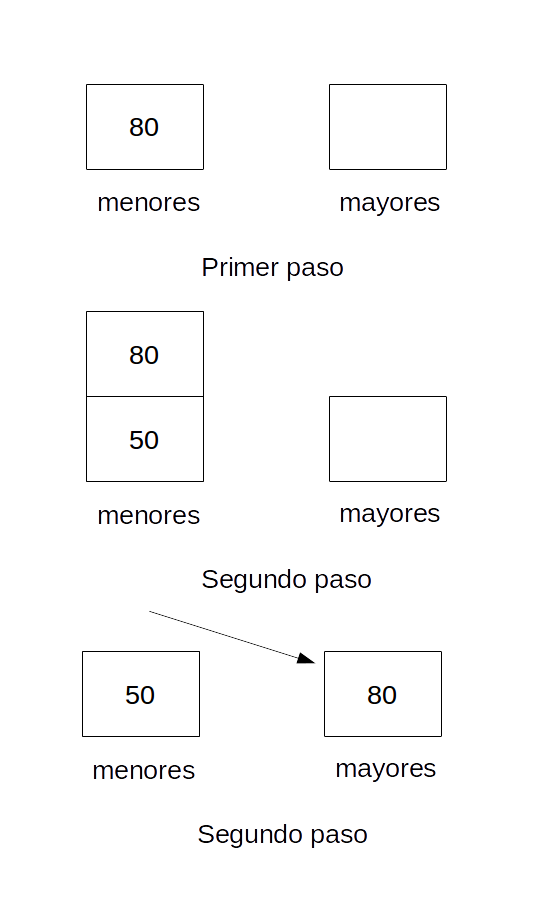
\includegraphics[width=0.45\textwidth]{imagenes/ej2-ejemplo.png}
\end{figure}

\newpage

Vemos en el primer paso se pone a 80 en menores ya que no hay ninguno más en las colas. En el segundo, el 50 es menor que el único valor de la cola menores. 
Por lo tanto se lo coloca en está y queda en el segundo lugar, pero entonces tenemos una cola con dos elementos y la otra con ninguno. Para resolver esto pasamos el 80
a la cola mayores y continua respetando su invariante. En el primer lugar la media es 80 (es el único que hay) y en el segundo es 65(80 + 50/2).


\subsection{Correctitud}


Podemos demostrar que el algoritmo es correcto por construcción.
Partiendo de una lista de números considerados vacía, al agregar el primero se lo coloca en una de las colas. Al tener una cantidad impar de números, el mediano es el próximo de la cola con mayor elementos, que en este caso es el mismo número, lo que es correcto. 

A partir de este punto, cada vez que se agrega un elemento, la cantidad de enteros considerados sera par e impar sucesivamente.
 En ambos casos, al agregar el número se lo insertará en la cola correspondiente, según sea mayor que el mínimo de la cola de enteros mayores a la mediana, o menor al máximo de la cola de menores a la mediana. 
Tras balancear las colas si fuera necesario, si la cantidad de números es par cada cola tiene la mitad de ellos. De esta manera, la mediana se calcula a partir de los próximos de cada cola y el resultado es correcto.
 Si fueran impares, el próximo de la cola con más elementos tiene exactamente la misma cantidad de enteros menores a el como mayores, por lo que el resultado del algoritmo es la mediana.

\begin{comment}
Para demostrar que el algoritmo usado es correcto utilizaremos indución sobre el tamaño del arreglo.

Quiero ver que: CB y ($\forall$ a : Lista(int))(P(a) $\Rightarrow$ ($\forall$ i : int)(P(AgregarAtras(a, i)))) 

Siendo P(a) = true $\Leftrightarrow$ aMedias(a) es igual a la respuesta correcta esperada por el algoritmo.

CB = P(b) donde b es una lista con un solo elemento.

CB = La lista soló tiene un elemento, cuando esto ocurra entrará en el primer si y pondra el elemento en el arreglo resultado. No entrará en la guarda del mientras y
con esto terminara. Devolviendo como resultado la mismo lista, esto es correcto ya que al soló haber un elemento el único mediano es el mismo.

Resuelto el caso base, pasemos ahora al paso inductivo. Supongamos que sabemos que vale para n elementos, osea que dandole un arreglo de n elementos devuelve el resultado correcto. Veamos ahora que vale para n + 1 elementos. 

Por hipotesis inductiva el resultado que nos da en n elementos es correcto y el arreglo de n + 1 elementos lo consideramos como agregarle un elemento al final del arreglo. Entonces irá construyendo el resultado correcto hasta llegar al último valor. Primero decidimos si pasarlo a la cola de menores o de mayores y si debemos reacomodarlas posteriormente.

Supongamos el caso de que n sea par, entonces al ponerlo en una de las dos colas no hay necesidad de más cambios en la estructura. Si el nuevo elemento es el mediano del arreglo entonces quedará como menor a todos los mayores y mayor a todos los menores. Entonces ese mismo será último del resultado. En caso contrario se irá o bien a la de menores o a la de mayores y el mediano se decidirá por los valores que ya hay en las colas. Como se va a la de mayores (o menores) entonces hay un elemento más que es mayor(o menor) al mediano. entonces el que quede en la cola con un elemento mayor que la otra será el resultado(Es impar). 

En el caso de que n sea impar, tenemos que al agregarlo en la respectiva estructura tendremos dos casos. Los cuales son si las desequilibra o si no.
Si las desequilibra, entonces se las tendrá que reacomodar pasando el próximo de la que tiene más elementos a la otra. Nos quedará dos colas con la misma cantidad de valores. Pero si o si uno de los próximos es el mediano anterior. El otro puede ser el ingresado o uno que estuviese anteriormente. Suponiendo que fuese uno anterior, entonces sabemos que es correcto por HI, ya que lo único que hará el nuevo es decidir si es el de menores o el de mayores. Esto último significa que tenemos un nuevo elemento que será el que sea o bien mayor de los menores o el menor de los mayores(de los que están en el medio). En el caso contrario, este es menor que todos los mayores o mayor que todos los mayores. Por lo tanto el último valor del resultado se hará sumando el mediano anterior con el nuevo elemento, lo cual es correcto por lo que sabemos de este.

Y con esto cubrimos todos los casos planteados y demostramos de forma semi-formal que el algoritmo es correcto.
\end{comment}
\subsection{Complejidad}
La complejidad del algoritmo es O(n log n) en el peor caso. 
Mientras que la complejidad pedida, por enunciado, es una estrictamente mejor a O($n^2$). Por lo tanto este cumple con lo pedido. 

Esto lo podemos ver porque el peso de la complejidad recae principalmente en las operaciones con las colas de prioridad, las mismas según la documentacion de java es 
O(log n) para la inserción y el borrado y O(1) para acceder al próximo. Con n cantidad de elementos. Tenemos un ciclo que se repite la cantidad de veces como el tamaño de 
la entrada, en este mismo realizamos unas pocas operaciones constantes y cuanto mucho dos inserciones y un borrado. Entonces la complejidad nos cuesta O(n log n) con n
la cantidad de elementos de la entrada.

\subsection{Experimentación}

Elegimos las siguientes entradas para experimentar la correctitud del ejercicio:

Caso1: 2 6 11 45 89 192

Caso2: 192 89 45 11 6 2

La primera viene siendo una en la cual los elementos están ordenados de menor a mayor, la segunda es al revés. Con esto podemos ver si funciona correctamente en el caso en que
la muestra tenga siempre que migrar entre las colas por cada elemento. 

Caso 3: 54 54 54 54 54 54

La tercera es simplemente una en la cual todos los elementos son iguales. Veremos que en este caso la entrada es igual a la salida, es un experimento sencillo para ver como se
comporta en este caso borde. 

Caso 4: 34 35 25 59 18 98

Caso 5: 98 18 59 25 35 34

\newpage

La cuarta tiene sus valores saltando de uno menor otro mayor y así sucesivamente, al revés en el último. Esto nos permite saber si funciona en un caso en el cual no se da muy
seguido la migración de elementos entre las colas.

Los experimentos anteriores se pueden corroborar usando AMediasTest.java.


Utilizando el archivo AMediasTestTiempo.java podemos calcular los tiempos de ejecución del algoritmo para muestras de gran tamaño. Utilizaremos tres entradas: peor caso, mejor caso y caso promedio
. El peor caso en este algoritmo es obviamente en el cual tengamos que reacomodar los elementos de las colas una mayor cantidad de veces, para lograr esto simplemente le 
daremos una muestra que esté ordenada (en nuestro caso de mayor a menor) y por ende siempre se la encolara en menores para, posteriormente, tener que pasar el próximo elemento
de esta a la de mayores. Para el mejor caso lo que buscamos es, contrario al anterior, que nunca tenga caiga en el caso de tener que reacomodar los valores de las colas, 
para esto la secuencia de valores deberá estar ordenada de tal forma que tengamos uno que vaya a la de mayores y el siguiente a la de menores y así sucesivamente. 
Ej: [50, 49, 51, 48, 52, 47]. Por último tenemos el caso promedio, para este simplemente nos generamos valores aleatorios usando el tipo Random.


\begin{figure}[H]
  \centering
  % GNUPLOT: LaTeX picture
\setlength{\unitlength}{0.240900pt}
\ifx\plotpoint\undefined\newsavebox{\plotpoint}\fi
\sbox{\plotpoint}{\rule[-0.200pt]{0.400pt}{0.400pt}}%
\begin{picture}(1500,900)(0,0)
\sbox{\plotpoint}{\rule[-0.200pt]{0.400pt}{0.400pt}}%
\put(151.0,131.0){\rule[-0.200pt]{4.818pt}{0.400pt}}
\put(131,131){\makebox(0,0)[r]{$0$}}
\put(1419.0,131.0){\rule[-0.200pt]{4.818pt}{0.400pt}}
\put(151.0,277.0){\rule[-0.200pt]{4.818pt}{0.400pt}}
\put(131,277){\makebox(0,0)[r]{$0.1$}}
\put(1419.0,277.0){\rule[-0.200pt]{4.818pt}{0.400pt}}
\put(151.0,422.0){\rule[-0.200pt]{4.818pt}{0.400pt}}
\put(131,422){\makebox(0,0)[r]{$0.2$}}
\put(1419.0,422.0){\rule[-0.200pt]{4.818pt}{0.400pt}}
\put(151.0,568.0){\rule[-0.200pt]{4.818pt}{0.400pt}}
\put(131,568){\makebox(0,0)[r]{$0.3$}}
\put(1419.0,568.0){\rule[-0.200pt]{4.818pt}{0.400pt}}
\put(151.0,713.0){\rule[-0.200pt]{4.818pt}{0.400pt}}
\put(131,713){\makebox(0,0)[r]{$0.4$}}
\put(1419.0,713.0){\rule[-0.200pt]{4.818pt}{0.400pt}}
\put(151.0,859.0){\rule[-0.200pt]{4.818pt}{0.400pt}}
\put(131,859){\makebox(0,0)[r]{$0.5$}}
\put(1419.0,859.0){\rule[-0.200pt]{4.818pt}{0.400pt}}
\put(151.0,131.0){\rule[-0.200pt]{0.400pt}{4.818pt}}
\put(151,90){\makebox(0,0){$100000$}}
\put(151.0,839.0){\rule[-0.200pt]{0.400pt}{4.818pt}}
\put(294.0,131.0){\rule[-0.200pt]{0.400pt}{4.818pt}}
\put(294,90){\makebox(0,0){$200000$}}
\put(294.0,839.0){\rule[-0.200pt]{0.400pt}{4.818pt}}
\put(437.0,131.0){\rule[-0.200pt]{0.400pt}{4.818pt}}
\put(437,90){\makebox(0,0){$300000$}}
\put(437.0,839.0){\rule[-0.200pt]{0.400pt}{4.818pt}}
\put(580.0,131.0){\rule[-0.200pt]{0.400pt}{4.818pt}}
\put(580,90){\makebox(0,0){$400000$}}
\put(580.0,839.0){\rule[-0.200pt]{0.400pt}{4.818pt}}
\put(723.0,131.0){\rule[-0.200pt]{0.400pt}{4.818pt}}
\put(723,90){\makebox(0,0){$500000$}}
\put(723.0,839.0){\rule[-0.200pt]{0.400pt}{4.818pt}}
\put(867.0,131.0){\rule[-0.200pt]{0.400pt}{4.818pt}}
\put(867,90){\makebox(0,0){$600000$}}
\put(867.0,839.0){\rule[-0.200pt]{0.400pt}{4.818pt}}
\put(1010.0,131.0){\rule[-0.200pt]{0.400pt}{4.818pt}}
\put(1010,90){\makebox(0,0){$700000$}}
\put(1010.0,839.0){\rule[-0.200pt]{0.400pt}{4.818pt}}
\put(1153.0,131.0){\rule[-0.200pt]{0.400pt}{4.818pt}}
\put(1153,90){\makebox(0,0){$800000$}}
\put(1153.0,839.0){\rule[-0.200pt]{0.400pt}{4.818pt}}
\put(1296.0,131.0){\rule[-0.200pt]{0.400pt}{4.818pt}}
\put(1296,90){\makebox(0,0){$900000$}}
\put(1296.0,839.0){\rule[-0.200pt]{0.400pt}{4.818pt}}
\put(1439.0,131.0){\rule[-0.200pt]{0.400pt}{4.818pt}}
\put(1439,90){\makebox(0,0){$1\times10^{6}$}}
\put(1439.0,839.0){\rule[-0.200pt]{0.400pt}{4.818pt}}
\put(151.0,131.0){\rule[-0.200pt]{0.400pt}{175.375pt}}
\put(151.0,131.0){\rule[-0.200pt]{310.279pt}{0.400pt}}
\put(1439.0,131.0){\rule[-0.200pt]{0.400pt}{175.375pt}}
\put(151.0,859.0){\rule[-0.200pt]{310.279pt}{0.400pt}}
\put(30,495){\makebox(0,0){\rotatebox{90}{Tiempo}}}
\put(795,29){\makebox(0,0){Cantidad de valores del arreglo}}
\put(1279,818){\makebox(0,0)[r]{Mejor caso}}
\put(1299.0,818.0){\rule[-0.200pt]{24.090pt}{0.400pt}}
\put(151,134){\usebox{\plotpoint}}
\put(164,133.67){\rule{3.132pt}{0.400pt}}
\multiput(164.00,133.17)(6.500,1.000){2}{\rule{1.566pt}{0.400pt}}
\put(151.0,134.0){\rule[-0.200pt]{3.132pt}{0.400pt}}
\put(216,134.67){\rule{3.132pt}{0.400pt}}
\multiput(216.00,134.17)(6.500,1.000){2}{\rule{1.566pt}{0.400pt}}
\put(177.0,135.0){\rule[-0.200pt]{9.395pt}{0.400pt}}
\put(255,135.67){\rule{3.132pt}{0.400pt}}
\multiput(255.00,135.17)(6.500,1.000){2}{\rule{1.566pt}{0.400pt}}
\put(229.0,136.0){\rule[-0.200pt]{6.263pt}{0.400pt}}
\put(294,136.67){\rule{3.132pt}{0.400pt}}
\multiput(294.00,136.17)(6.500,1.000){2}{\rule{1.566pt}{0.400pt}}
\put(268.0,137.0){\rule[-0.200pt]{6.263pt}{0.400pt}}
\put(346,137.67){\rule{3.132pt}{0.400pt}}
\multiput(346.00,137.17)(6.500,1.000){2}{\rule{1.566pt}{0.400pt}}
\put(307.0,138.0){\rule[-0.200pt]{9.395pt}{0.400pt}}
\put(385,138.67){\rule{3.132pt}{0.400pt}}
\multiput(385.00,138.17)(6.500,1.000){2}{\rule{1.566pt}{0.400pt}}
\put(359.0,139.0){\rule[-0.200pt]{6.263pt}{0.400pt}}
\put(437,139.67){\rule{3.132pt}{0.400pt}}
\multiput(437.00,139.17)(6.500,1.000){2}{\rule{1.566pt}{0.400pt}}
\put(398.0,140.0){\rule[-0.200pt]{9.395pt}{0.400pt}}
\put(476,140.67){\rule{3.132pt}{0.400pt}}
\multiput(476.00,140.17)(6.500,1.000){2}{\rule{1.566pt}{0.400pt}}
\put(450.0,141.0){\rule[-0.200pt]{6.263pt}{0.400pt}}
\put(515,141.67){\rule{3.132pt}{0.400pt}}
\multiput(515.00,141.17)(6.500,1.000){2}{\rule{1.566pt}{0.400pt}}
\put(489.0,142.0){\rule[-0.200pt]{6.263pt}{0.400pt}}
\put(567,142.67){\rule{3.132pt}{0.400pt}}
\multiput(567.00,142.17)(6.500,1.000){2}{\rule{1.566pt}{0.400pt}}
\put(528.0,143.0){\rule[-0.200pt]{9.395pt}{0.400pt}}
\put(606,143.67){\rule{3.132pt}{0.400pt}}
\multiput(606.00,143.17)(6.500,1.000){2}{\rule{1.566pt}{0.400pt}}
\put(580.0,144.0){\rule[-0.200pt]{6.263pt}{0.400pt}}
\put(645,144.67){\rule{3.132pt}{0.400pt}}
\multiput(645.00,144.17)(6.500,1.000){2}{\rule{1.566pt}{0.400pt}}
\put(619.0,145.0){\rule[-0.200pt]{6.263pt}{0.400pt}}
\put(684,145.67){\rule{3.132pt}{0.400pt}}
\multiput(684.00,145.17)(6.500,1.000){2}{\rule{1.566pt}{0.400pt}}
\put(658.0,146.0){\rule[-0.200pt]{6.263pt}{0.400pt}}
\put(736,146.67){\rule{3.132pt}{0.400pt}}
\multiput(736.00,146.17)(6.500,1.000){2}{\rule{1.566pt}{0.400pt}}
\put(697.0,147.0){\rule[-0.200pt]{9.395pt}{0.400pt}}
\put(775,147.67){\rule{3.132pt}{0.400pt}}
\multiput(775.00,147.17)(6.500,1.000){2}{\rule{1.566pt}{0.400pt}}
\put(749.0,148.0){\rule[-0.200pt]{6.263pt}{0.400pt}}
\put(815,148.67){\rule{3.132pt}{0.400pt}}
\multiput(815.00,148.17)(6.500,1.000){2}{\rule{1.566pt}{0.400pt}}
\put(788.0,149.0){\rule[-0.200pt]{6.504pt}{0.400pt}}
\put(854,149.67){\rule{3.132pt}{0.400pt}}
\multiput(854.00,149.17)(6.500,1.000){2}{\rule{1.566pt}{0.400pt}}
\put(828.0,150.0){\rule[-0.200pt]{6.263pt}{0.400pt}}
\put(893,150.67){\rule{3.132pt}{0.400pt}}
\multiput(893.00,150.17)(6.500,1.000){2}{\rule{1.566pt}{0.400pt}}
\put(867.0,151.0){\rule[-0.200pt]{6.263pt}{0.400pt}}
\put(945,151.67){\rule{3.132pt}{0.400pt}}
\multiput(945.00,151.17)(6.500,1.000){2}{\rule{1.566pt}{0.400pt}}
\put(906.0,152.0){\rule[-0.200pt]{9.395pt}{0.400pt}}
\put(984,152.67){\rule{3.132pt}{0.400pt}}
\multiput(984.00,152.17)(6.500,1.000){2}{\rule{1.566pt}{0.400pt}}
\put(958.0,153.0){\rule[-0.200pt]{6.263pt}{0.400pt}}
\put(1023,153.67){\rule{3.132pt}{0.400pt}}
\multiput(1023.00,153.17)(6.500,1.000){2}{\rule{1.566pt}{0.400pt}}
\put(997.0,154.0){\rule[-0.200pt]{6.263pt}{0.400pt}}
\put(1062,154.67){\rule{3.132pt}{0.400pt}}
\multiput(1062.00,154.17)(6.500,1.000){2}{\rule{1.566pt}{0.400pt}}
\put(1036.0,155.0){\rule[-0.200pt]{6.263pt}{0.400pt}}
\put(1101,155.67){\rule{3.132pt}{0.400pt}}
\multiput(1101.00,155.17)(6.500,1.000){2}{\rule{1.566pt}{0.400pt}}
\put(1075.0,156.0){\rule[-0.200pt]{6.263pt}{0.400pt}}
\put(1153,156.67){\rule{3.132pt}{0.400pt}}
\multiput(1153.00,156.17)(6.500,1.000){2}{\rule{1.566pt}{0.400pt}}
\put(1114.0,157.0){\rule[-0.200pt]{9.395pt}{0.400pt}}
\put(1192,157.67){\rule{3.132pt}{0.400pt}}
\multiput(1192.00,157.17)(6.500,1.000){2}{\rule{1.566pt}{0.400pt}}
\put(1166.0,158.0){\rule[-0.200pt]{6.263pt}{0.400pt}}
\put(1231,158.67){\rule{3.132pt}{0.400pt}}
\multiput(1231.00,158.17)(6.500,1.000){2}{\rule{1.566pt}{0.400pt}}
\put(1205.0,159.0){\rule[-0.200pt]{6.263pt}{0.400pt}}
\put(1270,159.67){\rule{3.132pt}{0.400pt}}
\multiput(1270.00,159.17)(6.500,1.000){2}{\rule{1.566pt}{0.400pt}}
\put(1244.0,160.0){\rule[-0.200pt]{6.263pt}{0.400pt}}
\put(1309,160.67){\rule{3.132pt}{0.400pt}}
\multiput(1309.00,160.17)(6.500,1.000){2}{\rule{1.566pt}{0.400pt}}
\put(1283.0,161.0){\rule[-0.200pt]{6.263pt}{0.400pt}}
\put(1348,161.67){\rule{3.132pt}{0.400pt}}
\multiput(1348.00,161.17)(6.500,1.000){2}{\rule{1.566pt}{0.400pt}}
\put(1322.0,162.0){\rule[-0.200pt]{6.263pt}{0.400pt}}
\put(1374,162.67){\rule{3.132pt}{0.400pt}}
\multiput(1374.00,162.17)(6.500,1.000){2}{\rule{1.566pt}{0.400pt}}
\put(1361.0,163.0){\rule[-0.200pt]{3.132pt}{0.400pt}}
\put(1413,163.67){\rule{3.132pt}{0.400pt}}
\multiput(1413.00,163.17)(6.500,1.000){2}{\rule{1.566pt}{0.400pt}}
\put(1387.0,164.0){\rule[-0.200pt]{6.263pt}{0.400pt}}
\put(1426.0,165.0){\rule[-0.200pt]{3.132pt}{0.400pt}}
\put(1279,777){\makebox(0,0)[r]{Peor caso}}
\multiput(1299,777)(20.756,0.000){5}{\usebox{\plotpoint}}
\put(1399,777){\usebox{\plotpoint}}
\put(151,146){\usebox{\plotpoint}}
\put(151.00,146.00){\usebox{\plotpoint}}
\put(171.69,147.59){\usebox{\plotpoint}}
\put(192.39,149.18){\usebox{\plotpoint}}
\put(213.00,151.54){\usebox{\plotpoint}}
\put(233.66,153.36){\usebox{\plotpoint}}
\put(254.36,154.95){\usebox{\plotpoint}}
\put(274.99,157.08){\usebox{\plotpoint}}
\put(295.63,159.13){\usebox{\plotpoint}}
\put(316.25,161.42){\usebox{\plotpoint}}
\put(336.91,163.30){\usebox{\plotpoint}}
\put(357.60,164.89){\usebox{\plotpoint}}
\put(378.18,167.48){\usebox{\plotpoint}}
\put(398.87,169.13){\usebox{\plotpoint}}
\put(419.46,171.65){\usebox{\plotpoint}}
\put(440.15,173.24){\usebox{\plotpoint}}
\put(460.75,175.65){\usebox{\plotpoint}}
\put(481.42,177.42){\usebox{\plotpoint}}
\put(502.00,180.00){\usebox{\plotpoint}}
\put(522.70,181.59){\usebox{\plotpoint}}
\put(543.28,184.18){\usebox{\plotpoint}}
\put(563.97,185.77){\usebox{\plotpoint}}
\put(584.63,187.71){\usebox{\plotpoint}}
\put(605.25,189.94){\usebox{\plotpoint}}
\put(625.88,192.06){\usebox{\plotpoint}}
\put(646.52,194.12){\usebox{\plotpoint}}
\put(667.14,196.41){\usebox{\plotpoint}}
\put(687.80,198.29){\usebox{\plotpoint}}
\put(708.39,200.75){\usebox{\plotpoint}}
\put(729.07,202.47){\usebox{\plotpoint}}
\put(749.65,205.05){\usebox{\plotpoint}}
\put(770.35,206.64){\usebox{\plotpoint}}
\put(790.93,209.21){\usebox{\plotpoint}}
\put(811.63,210.74){\usebox{\plotpoint}}
\put(832.21,213.32){\usebox{\plotpoint}}
\put(852.90,214.92){\usebox{\plotpoint}}
\put(873.48,217.50){\usebox{\plotpoint}}
\put(894.17,219.18){\usebox{\plotpoint}}
\put(914.76,221.67){\usebox{\plotpoint}}
\put(935.34,224.26){\usebox{\plotpoint}}
\put(956.03,225.85){\usebox{\plotpoint}}
\put(976.61,228.43){\usebox{\plotpoint}}
\put(997.30,230.05){\usebox{\plotpoint}}
\put(1017.88,232.61){\usebox{\plotpoint}}
\put(1038.56,234.39){\usebox{\plotpoint}}
\put(1059.16,236.78){\usebox{\plotpoint}}
\put(1079.74,239.36){\usebox{\plotpoint}}
\put(1100.43,240.96){\usebox{\plotpoint}}
\put(1121.01,243.54){\usebox{\plotpoint}}
\put(1141.59,246.12){\usebox{\plotpoint}}
\put(1162.29,247.71){\usebox{\plotpoint}}
\put(1182.87,250.30){\usebox{\plotpoint}}
\put(1203.46,252.76){\usebox{\plotpoint}}
\put(1224.14,254.47){\usebox{\plotpoint}}
\put(1244.72,257.06){\usebox{\plotpoint}}
\put(1265.34,259.28){\usebox{\plotpoint}}
\put(1286.00,261.23){\usebox{\plotpoint}}
\put(1306.60,263.63){\usebox{\plotpoint}}
\put(1327.27,265.41){\usebox{\plotpoint}}
\put(1347.85,267.98){\usebox{\plotpoint}}
\put(1368.48,270.15){\usebox{\plotpoint}}
\put(1389.13,272.16){\usebox{\plotpoint}}
\put(1409.74,274.50){\usebox{\plotpoint}}
\put(1430.36,276.67){\usebox{\plotpoint}}
\put(1439,278){\usebox{\plotpoint}}
\sbox{\plotpoint}{\rule[-0.400pt]{0.800pt}{0.800pt}}%
\sbox{\plotpoint}{\rule[-0.200pt]{0.400pt}{0.400pt}}%
\put(1279,736){\makebox(0,0)[r]{Caso promedio}}
\sbox{\plotpoint}{\rule[-0.400pt]{0.800pt}{0.800pt}}%
\put(1299.0,736.0){\rule[-0.400pt]{24.090pt}{0.800pt}}
\put(151,141){\usebox{\plotpoint}}
\put(151,139.84){\rule{3.132pt}{0.800pt}}
\multiput(151.00,139.34)(6.500,1.000){2}{\rule{1.566pt}{0.800pt}}
\put(164,140.84){\rule{3.132pt}{0.800pt}}
\multiput(164.00,140.34)(6.500,1.000){2}{\rule{1.566pt}{0.800pt}}
\put(177,141.84){\rule{3.132pt}{0.800pt}}
\multiput(177.00,141.34)(6.500,1.000){2}{\rule{1.566pt}{0.800pt}}
\put(190,142.84){\rule{3.132pt}{0.800pt}}
\multiput(190.00,142.34)(6.500,1.000){2}{\rule{1.566pt}{0.800pt}}
\put(203,143.84){\rule{3.132pt}{0.800pt}}
\multiput(203.00,143.34)(6.500,1.000){2}{\rule{1.566pt}{0.800pt}}
\put(216,144.84){\rule{3.132pt}{0.800pt}}
\multiput(216.00,144.34)(6.500,1.000){2}{\rule{1.566pt}{0.800pt}}
\put(229,145.84){\rule{3.132pt}{0.800pt}}
\multiput(229.00,145.34)(6.500,1.000){2}{\rule{1.566pt}{0.800pt}}
\put(242,146.84){\rule{3.132pt}{0.800pt}}
\multiput(242.00,146.34)(6.500,1.000){2}{\rule{1.566pt}{0.800pt}}
\put(268,147.84){\rule{3.132pt}{0.800pt}}
\multiput(268.00,147.34)(6.500,1.000){2}{\rule{1.566pt}{0.800pt}}
\put(281,148.84){\rule{3.132pt}{0.800pt}}
\multiput(281.00,148.34)(6.500,1.000){2}{\rule{1.566pt}{0.800pt}}
\put(294,149.84){\rule{3.132pt}{0.800pt}}
\multiput(294.00,149.34)(6.500,1.000){2}{\rule{1.566pt}{0.800pt}}
\put(307,150.84){\rule{3.132pt}{0.800pt}}
\multiput(307.00,150.34)(6.500,1.000){2}{\rule{1.566pt}{0.800pt}}
\put(320,151.84){\rule{3.132pt}{0.800pt}}
\multiput(320.00,151.34)(6.500,1.000){2}{\rule{1.566pt}{0.800pt}}
\put(333,152.84){\rule{3.132pt}{0.800pt}}
\multiput(333.00,152.34)(6.500,1.000){2}{\rule{1.566pt}{0.800pt}}
\put(346,153.84){\rule{3.132pt}{0.800pt}}
\multiput(346.00,153.34)(6.500,1.000){2}{\rule{1.566pt}{0.800pt}}
\put(359,154.84){\rule{3.132pt}{0.800pt}}
\multiput(359.00,154.34)(6.500,1.000){2}{\rule{1.566pt}{0.800pt}}
\put(372,155.84){\rule{3.132pt}{0.800pt}}
\multiput(372.00,155.34)(6.500,1.000){2}{\rule{1.566pt}{0.800pt}}
\put(385,156.84){\rule{3.132pt}{0.800pt}}
\multiput(385.00,156.34)(6.500,1.000){2}{\rule{1.566pt}{0.800pt}}
\put(398,157.84){\rule{3.132pt}{0.800pt}}
\multiput(398.00,157.34)(6.500,1.000){2}{\rule{1.566pt}{0.800pt}}
\put(411,158.84){\rule{3.132pt}{0.800pt}}
\multiput(411.00,158.34)(6.500,1.000){2}{\rule{1.566pt}{0.800pt}}
\put(424,159.84){\rule{3.132pt}{0.800pt}}
\multiput(424.00,159.34)(6.500,1.000){2}{\rule{1.566pt}{0.800pt}}
\put(437,160.84){\rule{3.132pt}{0.800pt}}
\multiput(437.00,160.34)(6.500,1.000){2}{\rule{1.566pt}{0.800pt}}
\put(450,161.84){\rule{3.132pt}{0.800pt}}
\multiput(450.00,161.34)(6.500,1.000){2}{\rule{1.566pt}{0.800pt}}
\put(463,162.84){\rule{3.132pt}{0.800pt}}
\multiput(463.00,162.34)(6.500,1.000){2}{\rule{1.566pt}{0.800pt}}
\put(476,163.84){\rule{3.132pt}{0.800pt}}
\multiput(476.00,163.34)(6.500,1.000){2}{\rule{1.566pt}{0.800pt}}
\put(489,164.84){\rule{3.132pt}{0.800pt}}
\multiput(489.00,164.34)(6.500,1.000){2}{\rule{1.566pt}{0.800pt}}
\put(502,165.84){\rule{3.132pt}{0.800pt}}
\multiput(502.00,165.34)(6.500,1.000){2}{\rule{1.566pt}{0.800pt}}
\put(515,166.84){\rule{3.132pt}{0.800pt}}
\multiput(515.00,166.34)(6.500,1.000){2}{\rule{1.566pt}{0.800pt}}
\put(528,167.84){\rule{3.132pt}{0.800pt}}
\multiput(528.00,167.34)(6.500,1.000){2}{\rule{1.566pt}{0.800pt}}
\put(541,168.84){\rule{3.132pt}{0.800pt}}
\multiput(541.00,168.34)(6.500,1.000){2}{\rule{1.566pt}{0.800pt}}
\put(554,169.84){\rule{3.132pt}{0.800pt}}
\multiput(554.00,169.34)(6.500,1.000){2}{\rule{1.566pt}{0.800pt}}
\put(567,170.84){\rule{3.132pt}{0.800pt}}
\multiput(567.00,170.34)(6.500,1.000){2}{\rule{1.566pt}{0.800pt}}
\put(580,171.84){\rule{3.132pt}{0.800pt}}
\multiput(580.00,171.34)(6.500,1.000){2}{\rule{1.566pt}{0.800pt}}
\put(593,172.84){\rule{3.132pt}{0.800pt}}
\multiput(593.00,172.34)(6.500,1.000){2}{\rule{1.566pt}{0.800pt}}
\put(606,173.84){\rule{3.132pt}{0.800pt}}
\multiput(606.00,173.34)(6.500,1.000){2}{\rule{1.566pt}{0.800pt}}
\put(619,174.84){\rule{3.132pt}{0.800pt}}
\multiput(619.00,174.34)(6.500,1.000){2}{\rule{1.566pt}{0.800pt}}
\put(632,175.84){\rule{3.132pt}{0.800pt}}
\multiput(632.00,175.34)(6.500,1.000){2}{\rule{1.566pt}{0.800pt}}
\put(645,176.84){\rule{3.132pt}{0.800pt}}
\multiput(645.00,176.34)(6.500,1.000){2}{\rule{1.566pt}{0.800pt}}
\put(658,177.84){\rule{3.132pt}{0.800pt}}
\multiput(658.00,177.34)(6.500,1.000){2}{\rule{1.566pt}{0.800pt}}
\put(671,178.84){\rule{3.132pt}{0.800pt}}
\multiput(671.00,178.34)(6.500,1.000){2}{\rule{1.566pt}{0.800pt}}
\put(684,179.84){\rule{3.132pt}{0.800pt}}
\multiput(684.00,179.34)(6.500,1.000){2}{\rule{1.566pt}{0.800pt}}
\put(697,180.84){\rule{3.132pt}{0.800pt}}
\multiput(697.00,180.34)(6.500,1.000){2}{\rule{1.566pt}{0.800pt}}
\put(255.0,149.0){\rule[-0.400pt]{3.132pt}{0.800pt}}
\put(723,181.84){\rule{3.132pt}{0.800pt}}
\multiput(723.00,181.34)(6.500,1.000){2}{\rule{1.566pt}{0.800pt}}
\put(736,182.84){\rule{3.132pt}{0.800pt}}
\multiput(736.00,182.34)(6.500,1.000){2}{\rule{1.566pt}{0.800pt}}
\put(749,183.84){\rule{3.132pt}{0.800pt}}
\multiput(749.00,183.34)(6.500,1.000){2}{\rule{1.566pt}{0.800pt}}
\put(762,184.84){\rule{3.132pt}{0.800pt}}
\multiput(762.00,184.34)(6.500,1.000){2}{\rule{1.566pt}{0.800pt}}
\put(775,185.84){\rule{3.132pt}{0.800pt}}
\multiput(775.00,185.34)(6.500,1.000){2}{\rule{1.566pt}{0.800pt}}
\put(788,186.84){\rule{3.373pt}{0.800pt}}
\multiput(788.00,186.34)(7.000,1.000){2}{\rule{1.686pt}{0.800pt}}
\put(802,187.84){\rule{3.132pt}{0.800pt}}
\multiput(802.00,187.34)(6.500,1.000){2}{\rule{1.566pt}{0.800pt}}
\put(815,188.84){\rule{3.132pt}{0.800pt}}
\multiput(815.00,188.34)(6.500,1.000){2}{\rule{1.566pt}{0.800pt}}
\put(828,189.84){\rule{3.132pt}{0.800pt}}
\multiput(828.00,189.34)(6.500,1.000){2}{\rule{1.566pt}{0.800pt}}
\put(841,190.84){\rule{3.132pt}{0.800pt}}
\multiput(841.00,190.34)(6.500,1.000){2}{\rule{1.566pt}{0.800pt}}
\put(854,191.84){\rule{3.132pt}{0.800pt}}
\multiput(854.00,191.34)(6.500,1.000){2}{\rule{1.566pt}{0.800pt}}
\put(867,192.84){\rule{3.132pt}{0.800pt}}
\multiput(867.00,192.34)(6.500,1.000){2}{\rule{1.566pt}{0.800pt}}
\put(880,193.84){\rule{3.132pt}{0.800pt}}
\multiput(880.00,193.34)(6.500,1.000){2}{\rule{1.566pt}{0.800pt}}
\put(893,194.84){\rule{3.132pt}{0.800pt}}
\multiput(893.00,194.34)(6.500,1.000){2}{\rule{1.566pt}{0.800pt}}
\put(906,195.84){\rule{3.132pt}{0.800pt}}
\multiput(906.00,195.34)(6.500,1.000){2}{\rule{1.566pt}{0.800pt}}
\put(919,196.84){\rule{3.132pt}{0.800pt}}
\multiput(919.00,196.34)(6.500,1.000){2}{\rule{1.566pt}{0.800pt}}
\put(932,197.84){\rule{3.132pt}{0.800pt}}
\multiput(932.00,197.34)(6.500,1.000){2}{\rule{1.566pt}{0.800pt}}
\put(945,198.84){\rule{3.132pt}{0.800pt}}
\multiput(945.00,198.34)(6.500,1.000){2}{\rule{1.566pt}{0.800pt}}
\put(958,199.84){\rule{3.132pt}{0.800pt}}
\multiput(958.00,199.34)(6.500,1.000){2}{\rule{1.566pt}{0.800pt}}
\put(971,200.84){\rule{3.132pt}{0.800pt}}
\multiput(971.00,200.34)(6.500,1.000){2}{\rule{1.566pt}{0.800pt}}
\put(984,201.84){\rule{3.132pt}{0.800pt}}
\multiput(984.00,201.34)(6.500,1.000){2}{\rule{1.566pt}{0.800pt}}
\put(997,202.84){\rule{3.132pt}{0.800pt}}
\multiput(997.00,202.34)(6.500,1.000){2}{\rule{1.566pt}{0.800pt}}
\put(1010,203.84){\rule{3.132pt}{0.800pt}}
\multiput(1010.00,203.34)(6.500,1.000){2}{\rule{1.566pt}{0.800pt}}
\put(1023,204.84){\rule{3.132pt}{0.800pt}}
\multiput(1023.00,204.34)(6.500,1.000){2}{\rule{1.566pt}{0.800pt}}
\put(1036,205.84){\rule{3.132pt}{0.800pt}}
\multiput(1036.00,205.34)(6.500,1.000){2}{\rule{1.566pt}{0.800pt}}
\put(1049,206.84){\rule{3.132pt}{0.800pt}}
\multiput(1049.00,206.34)(6.500,1.000){2}{\rule{1.566pt}{0.800pt}}
\put(1062,207.84){\rule{3.132pt}{0.800pt}}
\multiput(1062.00,207.34)(6.500,1.000){2}{\rule{1.566pt}{0.800pt}}
\put(1075,208.84){\rule{3.132pt}{0.800pt}}
\multiput(1075.00,208.34)(6.500,1.000){2}{\rule{1.566pt}{0.800pt}}
\put(1088,209.84){\rule{3.132pt}{0.800pt}}
\multiput(1088.00,209.34)(6.500,1.000){2}{\rule{1.566pt}{0.800pt}}
\put(1101,210.84){\rule{3.132pt}{0.800pt}}
\multiput(1101.00,210.34)(6.500,1.000){2}{\rule{1.566pt}{0.800pt}}
\put(1114,211.84){\rule{3.132pt}{0.800pt}}
\multiput(1114.00,211.34)(6.500,1.000){2}{\rule{1.566pt}{0.800pt}}
\put(1127,212.84){\rule{3.132pt}{0.800pt}}
\multiput(1127.00,212.34)(6.500,1.000){2}{\rule{1.566pt}{0.800pt}}
\put(1140,213.84){\rule{3.132pt}{0.800pt}}
\multiput(1140.00,213.34)(6.500,1.000){2}{\rule{1.566pt}{0.800pt}}
\put(1153,214.84){\rule{3.132pt}{0.800pt}}
\multiput(1153.00,214.34)(6.500,1.000){2}{\rule{1.566pt}{0.800pt}}
\put(1166,215.84){\rule{3.132pt}{0.800pt}}
\multiput(1166.00,215.34)(6.500,1.000){2}{\rule{1.566pt}{0.800pt}}
\put(1179,216.84){\rule{3.132pt}{0.800pt}}
\multiput(1179.00,216.34)(6.500,1.000){2}{\rule{1.566pt}{0.800pt}}
\put(1192,217.84){\rule{3.132pt}{0.800pt}}
\multiput(1192.00,217.34)(6.500,1.000){2}{\rule{1.566pt}{0.800pt}}
\put(1205,218.84){\rule{3.132pt}{0.800pt}}
\multiput(1205.00,218.34)(6.500,1.000){2}{\rule{1.566pt}{0.800pt}}
\put(1218,219.84){\rule{3.132pt}{0.800pt}}
\multiput(1218.00,219.34)(6.500,1.000){2}{\rule{1.566pt}{0.800pt}}
\put(1231,220.84){\rule{3.132pt}{0.800pt}}
\multiput(1231.00,220.34)(6.500,1.000){2}{\rule{1.566pt}{0.800pt}}
\put(1244,221.84){\rule{3.132pt}{0.800pt}}
\multiput(1244.00,221.34)(6.500,1.000){2}{\rule{1.566pt}{0.800pt}}
\put(1257,222.84){\rule{3.132pt}{0.800pt}}
\multiput(1257.00,222.34)(6.500,1.000){2}{\rule{1.566pt}{0.800pt}}
\put(1270,223.84){\rule{3.132pt}{0.800pt}}
\multiput(1270.00,223.34)(6.500,1.000){2}{\rule{1.566pt}{0.800pt}}
\put(1283,224.84){\rule{3.132pt}{0.800pt}}
\multiput(1283.00,224.34)(6.500,1.000){2}{\rule{1.566pt}{0.800pt}}
\put(1296,225.84){\rule{3.132pt}{0.800pt}}
\multiput(1296.00,225.34)(6.500,1.000){2}{\rule{1.566pt}{0.800pt}}
\put(1309,226.84){\rule{3.132pt}{0.800pt}}
\multiput(1309.00,226.34)(6.500,1.000){2}{\rule{1.566pt}{0.800pt}}
\put(1322,227.84){\rule{3.132pt}{0.800pt}}
\multiput(1322.00,227.34)(6.500,1.000){2}{\rule{1.566pt}{0.800pt}}
\put(1335,228.84){\rule{3.132pt}{0.800pt}}
\multiput(1335.00,228.34)(6.500,1.000){2}{\rule{1.566pt}{0.800pt}}
\put(1348,229.84){\rule{3.132pt}{0.800pt}}
\multiput(1348.00,229.34)(6.500,1.000){2}{\rule{1.566pt}{0.800pt}}
\put(1361,230.84){\rule{3.132pt}{0.800pt}}
\multiput(1361.00,230.34)(6.500,1.000){2}{\rule{1.566pt}{0.800pt}}
\put(1374,231.84){\rule{3.132pt}{0.800pt}}
\multiput(1374.00,231.34)(6.500,1.000){2}{\rule{1.566pt}{0.800pt}}
\put(1387,232.84){\rule{3.132pt}{0.800pt}}
\multiput(1387.00,232.34)(6.500,1.000){2}{\rule{1.566pt}{0.800pt}}
\put(1400,233.84){\rule{3.132pt}{0.800pt}}
\multiput(1400.00,233.34)(6.500,1.000){2}{\rule{1.566pt}{0.800pt}}
\put(1413,234.84){\rule{3.132pt}{0.800pt}}
\multiput(1413.00,234.34)(6.500,1.000){2}{\rule{1.566pt}{0.800pt}}
\put(1426,235.84){\rule{3.132pt}{0.800pt}}
\multiput(1426.00,235.34)(6.500,1.000){2}{\rule{1.566pt}{0.800pt}}
\put(710.0,183.0){\rule[-0.400pt]{3.132pt}{0.800pt}}
\sbox{\plotpoint}{\rule[-0.500pt]{1.000pt}{1.000pt}}%
\sbox{\plotpoint}{\rule[-0.200pt]{0.400pt}{0.400pt}}%
\put(1279,695){\makebox(0,0)[r]{O(n log(n))}}
\sbox{\plotpoint}{\rule[-0.500pt]{1.000pt}{1.000pt}}%
\multiput(1299,695)(20.756,0.000){5}{\usebox{\plotpoint}}
\put(1399,695){\usebox{\plotpoint}}
\put(151,154){\usebox{\plotpoint}}
\put(151.00,154.00){\usebox{\plotpoint}}
\put(171.33,158.13){\usebox{\plotpoint}}
\put(191.82,161.42){\usebox{\plotpoint}}
\put(212.17,165.41){\usebox{\plotpoint}}
\put(232.50,169.54){\usebox{\plotpoint}}
\put(253.01,172.69){\usebox{\plotpoint}}
\put(273.34,176.82){\usebox{\plotpoint}}
\put(293.67,180.92){\usebox{\plotpoint}}
\put(314.08,184.63){\usebox{\plotpoint}}
\put(334.49,188.34){\usebox{\plotpoint}}
\put(354.84,192.36){\usebox{\plotpoint}}
\put(375.16,196.49){\usebox{\plotpoint}}
\put(395.53,200.43){\usebox{\plotpoint}}
\put(415.93,204.14){\usebox{\plotpoint}}
\put(436.33,207.90){\usebox{\plotpoint}}
\put(456.66,212.02){\usebox{\plotpoint}}
\put(476.99,216.15){\usebox{\plotpoint}}
\put(497.38,219.93){\usebox{\plotpoint}}
\put(517.79,223.64){\usebox{\plotpoint}}
\put(538.16,227.56){\usebox{\plotpoint}}
\put(558.42,232.02){\usebox{\plotpoint}}
\put(578.81,235.82){\usebox{\plotpoint}}
\put(599.14,239.94){\usebox{\plotpoint}}
\put(619.46,244.11){\usebox{\plotpoint}}
\put(639.80,248.20){\usebox{\plotpoint}}
\put(660.12,252.33){\usebox{\plotpoint}}
\put(680.50,256.19){\usebox{\plotpoint}}
\put(700.78,260.58){\usebox{\plotpoint}}
\put(721.13,264.57){\usebox{\plotpoint}}
\put(741.54,268.28){\usebox{\plotpoint}}
\put(761.76,272.95){\usebox{\plotpoint}}
\put(782.17,276.66){\usebox{\plotpoint}}
\put(802.45,281.07){\usebox{\plotpoint}}
\put(822.85,284.81){\usebox{\plotpoint}}
\put(843.26,288.52){\usebox{\plotpoint}}
\put(863.49,293.19){\usebox{\plotpoint}}
\put(883.89,296.90){\usebox{\plotpoint}}
\put(904.12,301.57){\usebox{\plotpoint}}
\put(924.52,305.27){\usebox{\plotpoint}}
\put(944.75,309.94){\usebox{\plotpoint}}
\put(965.16,313.65){\usebox{\plotpoint}}
\put(985.40,318.22){\usebox{\plotpoint}}
\put(1005.79,322.03){\usebox{\plotpoint}}
\put(1026.06,326.47){\usebox{\plotpoint}}
\put(1046.42,330.40){\usebox{\plotpoint}}
\put(1066.71,334.72){\usebox{\plotpoint}}
\put(1087.05,338.78){\usebox{\plotpoint}}
\put(1107.28,343.45){\usebox{\plotpoint}}
\put(1127.68,347.16){\usebox{\plotpoint}}
\put(1147.91,351.82){\usebox{\plotpoint}}
\put(1168.32,355.53){\usebox{\plotpoint}}
\put(1188.54,360.20){\usebox{\plotpoint}}
\put(1208.95,363.91){\usebox{\plotpoint}}
\put(1229.17,368.58){\usebox{\plotpoint}}
\put(1249.47,372.84){\usebox{\plotpoint}}
\put(1269.80,376.95){\usebox{\plotpoint}}
\put(1290.03,381.62){\usebox{\plotpoint}}
\put(1310.44,385.33){\usebox{\plotpoint}}
\put(1330.66,390.00){\usebox{\plotpoint}}
\put(1351.07,393.71){\usebox{\plotpoint}}
\put(1371.29,398.37){\usebox{\plotpoint}}
\put(1391.58,402.70){\usebox{\plotpoint}}
\put(1411.92,406.75){\usebox{\plotpoint}}
\put(1432.15,411.42){\usebox{\plotpoint}}
\put(1439,413){\usebox{\plotpoint}}
\sbox{\plotpoint}{\rule[-0.200pt]{0.400pt}{0.400pt}}%
\put(151.0,131.0){\rule[-0.200pt]{0.400pt}{175.375pt}}
\put(151.0,131.0){\rule[-0.200pt]{310.279pt}{0.400pt}}
\put(1439.0,131.0){\rule[-0.200pt]{0.400pt}{175.375pt}}
\put(151.0,859.0){\rule[-0.200pt]{310.279pt}{0.400pt}}
\end{picture}

   %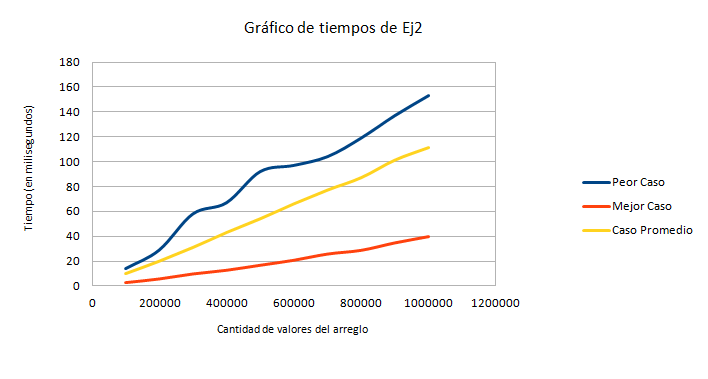
\includegraphics[width=1.1\textwidth]{imagenes/ExperimentoEj2.png}
  \caption{Tiempos de ejecución para ej.2}
\end{figure}


Como podemos ver el caso promedio está siempre acotado por el mejor y el peor caso(abajo y arriba respectivamente).
Se utilizaron muestras de esos tamaños simplemente porque eran lo suficientemente grandes como para que fueran apreciables los tiempos, pero a la vez no lo suficiente como para que replicar el experimente tardara excesivamente.
Para que las mediciones sean correctas, se repite el proceso para cada una de las muestras 100 veces y se toma el promedio de los tiempos. 

\begin{figure}[H]
  \centering
    % GNUPLOT: LaTeX picture
\setlength{\unitlength}{0.240900pt}
\ifx\plotpoint\undefined\newsavebox{\plotpoint}\fi
\begin{picture}(1500,900)(0,0)
\sbox{\plotpoint}{\rule[-0.200pt]{0.400pt}{0.400pt}}%
\put(231.0,131.0){\rule[-0.200pt]{4.818pt}{0.400pt}}
\put(211,131){\makebox(0,0)[r]{$0$}}
\put(1419.0,131.0){\rule[-0.200pt]{4.818pt}{0.400pt}}
\put(231.0,204.0){\rule[-0.200pt]{4.818pt}{0.400pt}}
\put(211,204){\makebox(0,0)[r]{$1\times10^{-13}$}}
\put(1419.0,204.0){\rule[-0.200pt]{4.818pt}{0.400pt}}
\put(231.0,277.0){\rule[-0.200pt]{4.818pt}{0.400pt}}
\put(211,277){\makebox(0,0)[r]{$2\times10^{-13}$}}
\put(1419.0,277.0){\rule[-0.200pt]{4.818pt}{0.400pt}}
\put(231.0,349.0){\rule[-0.200pt]{4.818pt}{0.400pt}}
\put(211,349){\makebox(0,0)[r]{$3\times10^{-13}$}}
\put(1419.0,349.0){\rule[-0.200pt]{4.818pt}{0.400pt}}
\put(231.0,422.0){\rule[-0.200pt]{4.818pt}{0.400pt}}
\put(211,422){\makebox(0,0)[r]{$4\times10^{-13}$}}
\put(1419.0,422.0){\rule[-0.200pt]{4.818pt}{0.400pt}}
\put(231.0,495.0){\rule[-0.200pt]{4.818pt}{0.400pt}}
\put(211,495){\makebox(0,0)[r]{$5\times10^{-13}$}}
\put(1419.0,495.0){\rule[-0.200pt]{4.818pt}{0.400pt}}
\put(231.0,568.0){\rule[-0.200pt]{4.818pt}{0.400pt}}
\put(211,568){\makebox(0,0)[r]{$6\times10^{-13}$}}
\put(1419.0,568.0){\rule[-0.200pt]{4.818pt}{0.400pt}}
\put(231.0,641.0){\rule[-0.200pt]{4.818pt}{0.400pt}}
\put(211,641){\makebox(0,0)[r]{$7\times10^{-13}$}}
\put(1419.0,641.0){\rule[-0.200pt]{4.818pt}{0.400pt}}
\put(231.0,713.0){\rule[-0.200pt]{4.818pt}{0.400pt}}
\put(211,713){\makebox(0,0)[r]{$8\times10^{-13}$}}
\put(1419.0,713.0){\rule[-0.200pt]{4.818pt}{0.400pt}}
\put(231.0,786.0){\rule[-0.200pt]{4.818pt}{0.400pt}}
\put(211,786){\makebox(0,0)[r]{$9\times10^{-13}$}}
\put(1419.0,786.0){\rule[-0.200pt]{4.818pt}{0.400pt}}
\put(231.0,859.0){\rule[-0.200pt]{4.818pt}{0.400pt}}
\put(211,859){\makebox(0,0)[r]{$1\times10^{-12}$}}
\put(1419.0,859.0){\rule[-0.200pt]{4.818pt}{0.400pt}}
\put(231.0,131.0){\rule[-0.200pt]{0.400pt}{4.818pt}}
\put(231,90){\makebox(0,0){$100000$}}
\put(231.0,839.0){\rule[-0.200pt]{0.400pt}{4.818pt}}
\put(365.0,131.0){\rule[-0.200pt]{0.400pt}{4.818pt}}
\put(365,90){\makebox(0,0){$200000$}}
\put(365.0,839.0){\rule[-0.200pt]{0.400pt}{4.818pt}}
\put(499.0,131.0){\rule[-0.200pt]{0.400pt}{4.818pt}}
\put(499,90){\makebox(0,0){$300000$}}
\put(499.0,839.0){\rule[-0.200pt]{0.400pt}{4.818pt}}
\put(634.0,131.0){\rule[-0.200pt]{0.400pt}{4.818pt}}
\put(634,90){\makebox(0,0){$400000$}}
\put(634.0,839.0){\rule[-0.200pt]{0.400pt}{4.818pt}}
\put(768.0,131.0){\rule[-0.200pt]{0.400pt}{4.818pt}}
\put(768,90){\makebox(0,0){$500000$}}
\put(768.0,839.0){\rule[-0.200pt]{0.400pt}{4.818pt}}
\put(902.0,131.0){\rule[-0.200pt]{0.400pt}{4.818pt}}
\put(902,90){\makebox(0,0){$600000$}}
\put(902.0,839.0){\rule[-0.200pt]{0.400pt}{4.818pt}}
\put(1036.0,131.0){\rule[-0.200pt]{0.400pt}{4.818pt}}
\put(1036,90){\makebox(0,0){$700000$}}
\put(1036.0,839.0){\rule[-0.200pt]{0.400pt}{4.818pt}}
\put(1171.0,131.0){\rule[-0.200pt]{0.400pt}{4.818pt}}
\put(1171,90){\makebox(0,0){$800000$}}
\put(1171.0,839.0){\rule[-0.200pt]{0.400pt}{4.818pt}}
\put(1305.0,131.0){\rule[-0.200pt]{0.400pt}{4.818pt}}
\put(1305,90){\makebox(0,0){$900000$}}
\put(1305.0,839.0){\rule[-0.200pt]{0.400pt}{4.818pt}}
\put(1439.0,131.0){\rule[-0.200pt]{0.400pt}{4.818pt}}
\put(1439,90){\makebox(0,0){$1\times10^{6}$}}
\put(1439.0,839.0){\rule[-0.200pt]{0.400pt}{4.818pt}}
\put(231.0,131.0){\rule[-0.200pt]{0.400pt}{175.375pt}}
\put(231.0,131.0){\rule[-0.200pt]{291.007pt}{0.400pt}}
\put(1439.0,131.0){\rule[-0.200pt]{0.400pt}{175.375pt}}
\put(231.0,859.0){\rule[-0.200pt]{291.007pt}{0.400pt}}
\put(30,495){\makebox(0,0){\rotatebox{90}{Tiempo}}}
\put(835,29){\makebox(0,0){Cantidad de valores del arreglo}}
\put(1279,818){\makebox(0,0)[r]{Mejor caso}}
\put(1299.0,818.0){\rule[-0.200pt]{24.090pt}{0.400pt}}
\put(231,282){\usebox{\plotpoint}}
\multiput(231.00,280.93)(1.033,-0.482){9}{\rule{0.900pt}{0.116pt}}
\multiput(231.00,281.17)(10.132,-6.000){2}{\rule{0.450pt}{0.400pt}}
\multiput(243.00,274.93)(1.033,-0.482){9}{\rule{0.900pt}{0.116pt}}
\multiput(243.00,275.17)(10.132,-6.000){2}{\rule{0.450pt}{0.400pt}}
\multiput(255.00,268.93)(1.123,-0.482){9}{\rule{0.967pt}{0.116pt}}
\multiput(255.00,269.17)(10.994,-6.000){2}{\rule{0.483pt}{0.400pt}}
\multiput(268.00,262.93)(1.033,-0.482){9}{\rule{0.900pt}{0.116pt}}
\multiput(268.00,263.17)(10.132,-6.000){2}{\rule{0.450pt}{0.400pt}}
\multiput(280.00,256.93)(1.267,-0.477){7}{\rule{1.060pt}{0.115pt}}
\multiput(280.00,257.17)(9.800,-5.000){2}{\rule{0.530pt}{0.400pt}}
\multiput(292.00,251.93)(1.267,-0.477){7}{\rule{1.060pt}{0.115pt}}
\multiput(292.00,252.17)(9.800,-5.000){2}{\rule{0.530pt}{0.400pt}}
\multiput(304.00,246.93)(1.267,-0.477){7}{\rule{1.060pt}{0.115pt}}
\multiput(304.00,247.17)(9.800,-5.000){2}{\rule{0.530pt}{0.400pt}}
\multiput(316.00,241.94)(1.797,-0.468){5}{\rule{1.400pt}{0.113pt}}
\multiput(316.00,242.17)(10.094,-4.000){2}{\rule{0.700pt}{0.400pt}}
\multiput(329.00,237.93)(1.267,-0.477){7}{\rule{1.060pt}{0.115pt}}
\multiput(329.00,238.17)(9.800,-5.000){2}{\rule{0.530pt}{0.400pt}}
\multiput(341.00,232.94)(1.651,-0.468){5}{\rule{1.300pt}{0.113pt}}
\multiput(341.00,233.17)(9.302,-4.000){2}{\rule{0.650pt}{0.400pt}}
\multiput(353.00,228.94)(1.651,-0.468){5}{\rule{1.300pt}{0.113pt}}
\multiput(353.00,229.17)(9.302,-4.000){2}{\rule{0.650pt}{0.400pt}}
\multiput(365.00,224.95)(2.472,-0.447){3}{\rule{1.700pt}{0.108pt}}
\multiput(365.00,225.17)(8.472,-3.000){2}{\rule{0.850pt}{0.400pt}}
\multiput(377.00,221.94)(1.797,-0.468){5}{\rule{1.400pt}{0.113pt}}
\multiput(377.00,222.17)(10.094,-4.000){2}{\rule{0.700pt}{0.400pt}}
\multiput(390.00,217.95)(2.472,-0.447){3}{\rule{1.700pt}{0.108pt}}
\multiput(390.00,218.17)(8.472,-3.000){2}{\rule{0.850pt}{0.400pt}}
\multiput(402.00,214.95)(2.472,-0.447){3}{\rule{1.700pt}{0.108pt}}
\multiput(402.00,215.17)(8.472,-3.000){2}{\rule{0.850pt}{0.400pt}}
\multiput(414.00,211.95)(2.472,-0.447){3}{\rule{1.700pt}{0.108pt}}
\multiput(414.00,212.17)(8.472,-3.000){2}{\rule{0.850pt}{0.400pt}}
\multiput(426.00,208.95)(2.472,-0.447){3}{\rule{1.700pt}{0.108pt}}
\multiput(426.00,209.17)(8.472,-3.000){2}{\rule{0.850pt}{0.400pt}}
\put(438,205.17){\rule{2.700pt}{0.400pt}}
\multiput(438.00,206.17)(7.396,-2.000){2}{\rule{1.350pt}{0.400pt}}
\multiput(451.00,203.95)(2.472,-0.447){3}{\rule{1.700pt}{0.108pt}}
\multiput(451.00,204.17)(8.472,-3.000){2}{\rule{0.850pt}{0.400pt}}
\put(463,200.17){\rule{2.500pt}{0.400pt}}
\multiput(463.00,201.17)(6.811,-2.000){2}{\rule{1.250pt}{0.400pt}}
\multiput(475.00,198.95)(2.472,-0.447){3}{\rule{1.700pt}{0.108pt}}
\multiput(475.00,199.17)(8.472,-3.000){2}{\rule{0.850pt}{0.400pt}}
\put(487,195.17){\rule{2.500pt}{0.400pt}}
\multiput(487.00,196.17)(6.811,-2.000){2}{\rule{1.250pt}{0.400pt}}
\put(499,193.17){\rule{2.700pt}{0.400pt}}
\multiput(499.00,194.17)(7.396,-2.000){2}{\rule{1.350pt}{0.400pt}}
\put(512,191.17){\rule{2.500pt}{0.400pt}}
\multiput(512.00,192.17)(6.811,-2.000){2}{\rule{1.250pt}{0.400pt}}
\put(524,189.17){\rule{2.500pt}{0.400pt}}
\multiput(524.00,190.17)(6.811,-2.000){2}{\rule{1.250pt}{0.400pt}}
\put(536,187.67){\rule{2.891pt}{0.400pt}}
\multiput(536.00,188.17)(6.000,-1.000){2}{\rule{1.445pt}{0.400pt}}
\put(548,186.17){\rule{2.500pt}{0.400pt}}
\multiput(548.00,187.17)(6.811,-2.000){2}{\rule{1.250pt}{0.400pt}}
\put(560,184.17){\rule{2.700pt}{0.400pt}}
\multiput(560.00,185.17)(7.396,-2.000){2}{\rule{1.350pt}{0.400pt}}
\put(573,182.67){\rule{2.891pt}{0.400pt}}
\multiput(573.00,183.17)(6.000,-1.000){2}{\rule{1.445pt}{0.400pt}}
\put(585,181.17){\rule{2.500pt}{0.400pt}}
\multiput(585.00,182.17)(6.811,-2.000){2}{\rule{1.250pt}{0.400pt}}
\put(597,179.67){\rule{2.891pt}{0.400pt}}
\multiput(597.00,180.17)(6.000,-1.000){2}{\rule{1.445pt}{0.400pt}}
\put(609,178.67){\rule{2.891pt}{0.400pt}}
\multiput(609.00,179.17)(6.000,-1.000){2}{\rule{1.445pt}{0.400pt}}
\put(621,177.17){\rule{2.700pt}{0.400pt}}
\multiput(621.00,178.17)(7.396,-2.000){2}{\rule{1.350pt}{0.400pt}}
\put(634,175.67){\rule{2.891pt}{0.400pt}}
\multiput(634.00,176.17)(6.000,-1.000){2}{\rule{1.445pt}{0.400pt}}
\put(646,174.67){\rule{2.891pt}{0.400pt}}
\multiput(646.00,175.17)(6.000,-1.000){2}{\rule{1.445pt}{0.400pt}}
\put(658,173.67){\rule{2.891pt}{0.400pt}}
\multiput(658.00,174.17)(6.000,-1.000){2}{\rule{1.445pt}{0.400pt}}
\put(670,172.67){\rule{2.891pt}{0.400pt}}
\multiput(670.00,173.17)(6.000,-1.000){2}{\rule{1.445pt}{0.400pt}}
\put(682,171.67){\rule{3.132pt}{0.400pt}}
\multiput(682.00,172.17)(6.500,-1.000){2}{\rule{1.566pt}{0.400pt}}
\put(695,170.67){\rule{2.891pt}{0.400pt}}
\multiput(695.00,171.17)(6.000,-1.000){2}{\rule{1.445pt}{0.400pt}}
\put(707,169.67){\rule{2.891pt}{0.400pt}}
\multiput(707.00,170.17)(6.000,-1.000){2}{\rule{1.445pt}{0.400pt}}
\put(719,168.67){\rule{2.891pt}{0.400pt}}
\multiput(719.00,169.17)(6.000,-1.000){2}{\rule{1.445pt}{0.400pt}}
\put(731,167.67){\rule{2.891pt}{0.400pt}}
\multiput(731.00,168.17)(6.000,-1.000){2}{\rule{1.445pt}{0.400pt}}
\put(756,166.67){\rule{2.891pt}{0.400pt}}
\multiput(756.00,167.17)(6.000,-1.000){2}{\rule{1.445pt}{0.400pt}}
\put(768,165.67){\rule{2.891pt}{0.400pt}}
\multiput(768.00,166.17)(6.000,-1.000){2}{\rule{1.445pt}{0.400pt}}
\put(780,164.67){\rule{2.891pt}{0.400pt}}
\multiput(780.00,165.17)(6.000,-1.000){2}{\rule{1.445pt}{0.400pt}}
\put(743.0,168.0){\rule[-0.200pt]{3.132pt}{0.400pt}}
\put(804,163.67){\rule{3.132pt}{0.400pt}}
\multiput(804.00,164.17)(6.500,-1.000){2}{\rule{1.566pt}{0.400pt}}
\put(817,162.67){\rule{2.891pt}{0.400pt}}
\multiput(817.00,163.17)(6.000,-1.000){2}{\rule{1.445pt}{0.400pt}}
\put(792.0,165.0){\rule[-0.200pt]{2.891pt}{0.400pt}}
\put(841,161.67){\rule{2.891pt}{0.400pt}}
\multiput(841.00,162.17)(6.000,-1.000){2}{\rule{1.445pt}{0.400pt}}
\put(829.0,163.0){\rule[-0.200pt]{2.891pt}{0.400pt}}
\put(866,160.67){\rule{2.891pt}{0.400pt}}
\multiput(866.00,161.17)(6.000,-1.000){2}{\rule{1.445pt}{0.400pt}}
\put(853.0,162.0){\rule[-0.200pt]{3.132pt}{0.400pt}}
\put(890,159.67){\rule{2.891pt}{0.400pt}}
\multiput(890.00,160.17)(6.000,-1.000){2}{\rule{1.445pt}{0.400pt}}
\put(878.0,161.0){\rule[-0.200pt]{2.891pt}{0.400pt}}
\put(914,158.67){\rule{3.132pt}{0.400pt}}
\multiput(914.00,159.17)(6.500,-1.000){2}{\rule{1.566pt}{0.400pt}}
\put(902.0,160.0){\rule[-0.200pt]{2.891pt}{0.400pt}}
\put(939,157.67){\rule{2.891pt}{0.400pt}}
\multiput(939.00,158.17)(6.000,-1.000){2}{\rule{1.445pt}{0.400pt}}
\put(927.0,159.0){\rule[-0.200pt]{2.891pt}{0.400pt}}
\put(963,156.67){\rule{2.891pt}{0.400pt}}
\multiput(963.00,157.17)(6.000,-1.000){2}{\rule{1.445pt}{0.400pt}}
\put(951.0,158.0){\rule[-0.200pt]{2.891pt}{0.400pt}}
\put(988,155.67){\rule{2.891pt}{0.400pt}}
\multiput(988.00,156.17)(6.000,-1.000){2}{\rule{1.445pt}{0.400pt}}
\put(975.0,157.0){\rule[-0.200pt]{3.132pt}{0.400pt}}
\put(1024,154.67){\rule{2.891pt}{0.400pt}}
\multiput(1024.00,155.17)(6.000,-1.000){2}{\rule{1.445pt}{0.400pt}}
\put(1000.0,156.0){\rule[-0.200pt]{5.782pt}{0.400pt}}
\put(1049,153.67){\rule{2.891pt}{0.400pt}}
\multiput(1049.00,154.17)(6.000,-1.000){2}{\rule{1.445pt}{0.400pt}}
\put(1036.0,155.0){\rule[-0.200pt]{3.132pt}{0.400pt}}
\put(1073,152.67){\rule{2.891pt}{0.400pt}}
\multiput(1073.00,153.17)(6.000,-1.000){2}{\rule{1.445pt}{0.400pt}}
\put(1061.0,154.0){\rule[-0.200pt]{2.891pt}{0.400pt}}
\put(1110,151.67){\rule{2.891pt}{0.400pt}}
\multiput(1110.00,152.17)(6.000,-1.000){2}{\rule{1.445pt}{0.400pt}}
\put(1085.0,153.0){\rule[-0.200pt]{6.022pt}{0.400pt}}
\put(1134,150.67){\rule{2.891pt}{0.400pt}}
\multiput(1134.00,151.17)(6.000,-1.000){2}{\rule{1.445pt}{0.400pt}}
\put(1122.0,152.0){\rule[-0.200pt]{2.891pt}{0.400pt}}
\put(1158,149.67){\rule{3.132pt}{0.400pt}}
\multiput(1158.00,150.17)(6.500,-1.000){2}{\rule{1.566pt}{0.400pt}}
\put(1146.0,151.0){\rule[-0.200pt]{2.891pt}{0.400pt}}
\put(1183,148.67){\rule{2.891pt}{0.400pt}}
\multiput(1183.00,149.17)(6.000,-1.000){2}{\rule{1.445pt}{0.400pt}}
\put(1171.0,150.0){\rule[-0.200pt]{2.891pt}{0.400pt}}
\put(1207,147.67){\rule{2.891pt}{0.400pt}}
\multiput(1207.00,148.17)(6.000,-1.000){2}{\rule{1.445pt}{0.400pt}}
\put(1195.0,149.0){\rule[-0.200pt]{2.891pt}{0.400pt}}
\put(1232,146.67){\rule{2.891pt}{0.400pt}}
\multiput(1232.00,147.17)(6.000,-1.000){2}{\rule{1.445pt}{0.400pt}}
\put(1219.0,148.0){\rule[-0.200pt]{3.132pt}{0.400pt}}
\put(1256,145.67){\rule{2.891pt}{0.400pt}}
\multiput(1256.00,146.17)(6.000,-1.000){2}{\rule{1.445pt}{0.400pt}}
\put(1268,144.67){\rule{2.891pt}{0.400pt}}
\multiput(1268.00,145.17)(6.000,-1.000){2}{\rule{1.445pt}{0.400pt}}
\put(1244.0,147.0){\rule[-0.200pt]{2.891pt}{0.400pt}}
\put(1293,143.67){\rule{2.891pt}{0.400pt}}
\multiput(1293.00,144.17)(6.000,-1.000){2}{\rule{1.445pt}{0.400pt}}
\put(1305,142.67){\rule{2.891pt}{0.400pt}}
\multiput(1305.00,143.17)(6.000,-1.000){2}{\rule{1.445pt}{0.400pt}}
\put(1317,141.67){\rule{2.891pt}{0.400pt}}
\multiput(1317.00,142.17)(6.000,-1.000){2}{\rule{1.445pt}{0.400pt}}
\put(1329,140.67){\rule{2.891pt}{0.400pt}}
\multiput(1329.00,141.17)(6.000,-1.000){2}{\rule{1.445pt}{0.400pt}}
\put(1341,139.67){\rule{3.132pt}{0.400pt}}
\multiput(1341.00,140.17)(6.500,-1.000){2}{\rule{1.566pt}{0.400pt}}
\put(1354,138.67){\rule{2.891pt}{0.400pt}}
\multiput(1354.00,139.17)(6.000,-1.000){2}{\rule{1.445pt}{0.400pt}}
\put(1366,137.67){\rule{2.891pt}{0.400pt}}
\multiput(1366.00,138.17)(6.000,-1.000){2}{\rule{1.445pt}{0.400pt}}
\put(1378,136.67){\rule{2.891pt}{0.400pt}}
\multiput(1378.00,137.17)(6.000,-1.000){2}{\rule{1.445pt}{0.400pt}}
\put(1390,135.17){\rule{2.500pt}{0.400pt}}
\multiput(1390.00,136.17)(6.811,-2.000){2}{\rule{1.250pt}{0.400pt}}
\put(1402,133.67){\rule{3.132pt}{0.400pt}}
\multiput(1402.00,134.17)(6.500,-1.000){2}{\rule{1.566pt}{0.400pt}}
\put(1415,132.67){\rule{2.891pt}{0.400pt}}
\multiput(1415.00,133.17)(6.000,-1.000){2}{\rule{1.445pt}{0.400pt}}
\put(1427,131.17){\rule{2.500pt}{0.400pt}}
\multiput(1427.00,132.17)(6.811,-2.000){2}{\rule{1.250pt}{0.400pt}}
\put(1280.0,145.0){\rule[-0.200pt]{3.132pt}{0.400pt}}
\put(1279,777){\makebox(0,0)[r]{Peor caso}}
\multiput(1299,777)(20.756,0.000){5}{\usebox{\plotpoint}}
\put(1399,777){\usebox{\plotpoint}}
\multiput(233,859)(6.766,-19.622){2}{\usebox{\plotpoint}}
\multiput(243,830)(7.093,-19.506){2}{\usebox{\plotpoint}}
\put(261.66,781.11){\usebox{\plotpoint}}
\multiput(268,766)(7.936,-19.178){2}{\usebox{\plotpoint}}
\put(285.89,723.75){\usebox{\plotpoint}}
\multiput(292,710)(8.698,-18.845){2}{\usebox{\plotpoint}}
\put(312.04,667.25){\usebox{\plotpoint}}
\put(321.71,648.89){\usebox{\plotpoint}}
\put(331.95,630.84){\usebox{\plotpoint}}
\multiput(341,615)(10.298,-18.021){2}{\usebox{\plotpoint}}
\put(363.59,577.23){\usebox{\plotpoint}}
\put(375.05,559.92){\usebox{\plotpoint}}
\put(387.47,543.30){\usebox{\plotpoint}}
\put(399.57,526.44){\usebox{\plotpoint}}
\put(412.33,510.08){\usebox{\plotpoint}}
\put(425.77,494.27){\usebox{\plotpoint}}
\put(439.39,478.61){\usebox{\plotpoint}}
\put(454.07,463.93){\usebox{\plotpoint}}
\put(468.74,449.26){\usebox{\plotpoint}}
\put(483.78,434.95){\usebox{\plotpoint}}
\put(499.61,421.53){\usebox{\plotpoint}}
\put(516.09,408.93){\usebox{\plotpoint}}
\put(532.70,396.48){\usebox{\plotpoint}}
\put(549.84,384.78){\usebox{\plotpoint}}
\put(567.52,373.95){\usebox{\plotpoint}}
\put(585.10,362.95){\usebox{\plotpoint}}
\put(603.43,353.25){\usebox{\plotpoint}}
\put(621.81,343.63){\usebox{\plotpoint}}
\put(640.77,335.18){\usebox{\plotpoint}}
\put(659.54,326.36){\usebox{\plotpoint}}
\put(678.94,319.02){\usebox{\plotpoint}}
\put(698.42,311.86){\usebox{\plotpoint}}
\put(717.81,304.50){\usebox{\plotpoint}}
\put(737.61,298.35){\usebox{\plotpoint}}
\put(757.52,292.49){\usebox{\plotpoint}}
\put(777.42,286.65){\usebox{\plotpoint}}
\put(797.55,281.61){\usebox{\plotpoint}}
\put(817.75,276.81){\usebox{\plotpoint}}
\put(837.88,271.78){\usebox{\plotpoint}}
\put(858.11,267.21){\usebox{\plotpoint}}
\put(878.40,262.93){\usebox{\plotpoint}}
\put(898.87,259.52){\usebox{\plotpoint}}
\put(919.36,256.18){\usebox{\plotpoint}}
\put(939.85,252.86){\usebox{\plotpoint}}
\put(960.32,249.45){\usebox{\plotpoint}}
\put(980.80,246.11){\usebox{\plotpoint}}
\put(1001.30,242.89){\usebox{\plotpoint}}
\put(1021.89,240.35){\usebox{\plotpoint}}
\put(1042.43,237.51){\usebox{\plotpoint}}
\put(1062.99,234.83){\usebox{\plotpoint}}
\put(1083.68,233.11){\usebox{\plotpoint}}
\put(1104.24,230.44){\usebox{\plotpoint}}
\put(1124.90,228.52){\usebox{\plotpoint}}
\put(1145.49,226.04){\usebox{\plotpoint}}
\put(1166.17,224.37){\usebox{\plotpoint}}
\put(1186.86,222.68){\usebox{\plotpoint}}
\put(1207.54,220.95){\usebox{\plotpoint}}
\put(1228.23,219.29){\usebox{\plotpoint}}
\put(1248.92,217.59){\usebox{\plotpoint}}
\put(1269.60,215.87){\usebox{\plotpoint}}
\put(1290.29,214.21){\usebox{\plotpoint}}
\put(1310.98,212.50){\usebox{\plotpoint}}
\put(1331.66,210.78){\usebox{\plotpoint}}
\put(1352.38,210.00){\usebox{\plotpoint}}
\put(1373.07,208.41){\usebox{\plotpoint}}
\put(1393.76,206.69){\usebox{\plotpoint}}
\put(1414.48,206.00){\usebox{\plotpoint}}
\put(1435.17,204.32){\usebox{\plotpoint}}
\put(1439,204){\usebox{\plotpoint}}
\sbox{\plotpoint}{\rule[-0.400pt]{0.800pt}{0.800pt}}%
\sbox{\plotpoint}{\rule[-0.200pt]{0.400pt}{0.400pt}}%
\put(1279,736){\makebox(0,0)[r]{Caso promedio}}
\sbox{\plotpoint}{\rule[-0.400pt]{0.800pt}{0.800pt}}%
\put(1299.0,736.0){\rule[-0.400pt]{24.090pt}{0.800pt}}
\put(231,630){\usebox{\plotpoint}}
\multiput(232.41,623.36)(0.511,-0.897){17}{\rule{0.123pt}{1.600pt}}
\multiput(229.34,626.68)(12.000,-17.679){2}{\rule{0.800pt}{0.800pt}}
\multiput(244.41,602.36)(0.511,-0.897){17}{\rule{0.123pt}{1.600pt}}
\multiput(241.34,605.68)(12.000,-17.679){2}{\rule{0.800pt}{0.800pt}}
\multiput(256.41,582.06)(0.509,-0.781){19}{\rule{0.123pt}{1.431pt}}
\multiput(253.34,585.03)(13.000,-17.030){2}{\rule{0.800pt}{0.715pt}}
\multiput(269.41,562.19)(0.511,-0.762){17}{\rule{0.123pt}{1.400pt}}
\multiput(266.34,565.09)(12.000,-15.094){2}{\rule{0.800pt}{0.700pt}}
\multiput(281.41,544.19)(0.511,-0.762){17}{\rule{0.123pt}{1.400pt}}
\multiput(278.34,547.09)(12.000,-15.094){2}{\rule{0.800pt}{0.700pt}}
\multiput(293.41,526.74)(0.511,-0.671){17}{\rule{0.123pt}{1.267pt}}
\multiput(290.34,529.37)(12.000,-13.371){2}{\rule{0.800pt}{0.633pt}}
\multiput(305.41,510.74)(0.511,-0.671){17}{\rule{0.123pt}{1.267pt}}
\multiput(302.34,513.37)(12.000,-13.371){2}{\rule{0.800pt}{0.633pt}}
\multiput(317.41,495.34)(0.509,-0.574){19}{\rule{0.123pt}{1.123pt}}
\multiput(314.34,497.67)(13.000,-12.669){2}{\rule{0.800pt}{0.562pt}}
\multiput(330.41,480.30)(0.511,-0.581){17}{\rule{0.123pt}{1.133pt}}
\multiput(327.34,482.65)(12.000,-11.648){2}{\rule{0.800pt}{0.567pt}}
\multiput(342.41,466.30)(0.511,-0.581){17}{\rule{0.123pt}{1.133pt}}
\multiput(339.34,468.65)(12.000,-11.648){2}{\rule{0.800pt}{0.567pt}}
\multiput(353.00,455.08)(0.491,-0.511){17}{\rule{1.000pt}{0.123pt}}
\multiput(353.00,455.34)(9.924,-12.000){2}{\rule{0.500pt}{0.800pt}}
\multiput(365.00,443.08)(0.491,-0.511){17}{\rule{1.000pt}{0.123pt}}
\multiput(365.00,443.34)(9.924,-12.000){2}{\rule{0.500pt}{0.800pt}}
\multiput(377.00,431.08)(0.536,-0.511){17}{\rule{1.067pt}{0.123pt}}
\multiput(377.00,431.34)(10.786,-12.000){2}{\rule{0.533pt}{0.800pt}}
\multiput(390.00,419.08)(0.539,-0.512){15}{\rule{1.073pt}{0.123pt}}
\multiput(390.00,419.34)(9.774,-11.000){2}{\rule{0.536pt}{0.800pt}}
\multiput(402.00,408.08)(0.599,-0.514){13}{\rule{1.160pt}{0.124pt}}
\multiput(402.00,408.34)(9.592,-10.000){2}{\rule{0.580pt}{0.800pt}}
\multiput(414.00,398.08)(0.599,-0.514){13}{\rule{1.160pt}{0.124pt}}
\multiput(414.00,398.34)(9.592,-10.000){2}{\rule{0.580pt}{0.800pt}}
\multiput(426.00,388.08)(0.674,-0.516){11}{\rule{1.267pt}{0.124pt}}
\multiput(426.00,388.34)(9.371,-9.000){2}{\rule{0.633pt}{0.800pt}}
\multiput(438.00,379.08)(0.737,-0.516){11}{\rule{1.356pt}{0.124pt}}
\multiput(438.00,379.34)(10.186,-9.000){2}{\rule{0.678pt}{0.800pt}}
\multiput(451.00,370.08)(0.774,-0.520){9}{\rule{1.400pt}{0.125pt}}
\multiput(451.00,370.34)(9.094,-8.000){2}{\rule{0.700pt}{0.800pt}}
\multiput(463.00,362.08)(0.774,-0.520){9}{\rule{1.400pt}{0.125pt}}
\multiput(463.00,362.34)(9.094,-8.000){2}{\rule{0.700pt}{0.800pt}}
\multiput(475.00,354.08)(0.913,-0.526){7}{\rule{1.571pt}{0.127pt}}
\multiput(475.00,354.34)(8.738,-7.000){2}{\rule{0.786pt}{0.800pt}}
\multiput(487.00,347.08)(0.913,-0.526){7}{\rule{1.571pt}{0.127pt}}
\multiput(487.00,347.34)(8.738,-7.000){2}{\rule{0.786pt}{0.800pt}}
\multiput(499.00,340.08)(1.000,-0.526){7}{\rule{1.686pt}{0.127pt}}
\multiput(499.00,340.34)(9.501,-7.000){2}{\rule{0.843pt}{0.800pt}}
\multiput(512.00,333.08)(0.913,-0.526){7}{\rule{1.571pt}{0.127pt}}
\multiput(512.00,333.34)(8.738,-7.000){2}{\rule{0.786pt}{0.800pt}}
\multiput(524.00,326.07)(1.132,-0.536){5}{\rule{1.800pt}{0.129pt}}
\multiput(524.00,326.34)(8.264,-6.000){2}{\rule{0.900pt}{0.800pt}}
\multiput(536.00,320.06)(1.600,-0.560){3}{\rule{2.120pt}{0.135pt}}
\multiput(536.00,320.34)(7.600,-5.000){2}{\rule{1.060pt}{0.800pt}}
\multiput(548.00,315.07)(1.132,-0.536){5}{\rule{1.800pt}{0.129pt}}
\multiput(548.00,315.34)(8.264,-6.000){2}{\rule{0.900pt}{0.800pt}}
\multiput(560.00,309.06)(1.768,-0.560){3}{\rule{2.280pt}{0.135pt}}
\multiput(560.00,309.34)(8.268,-5.000){2}{\rule{1.140pt}{0.800pt}}
\multiput(573.00,304.06)(1.600,-0.560){3}{\rule{2.120pt}{0.135pt}}
\multiput(573.00,304.34)(7.600,-5.000){2}{\rule{1.060pt}{0.800pt}}
\multiput(585.00,299.06)(1.600,-0.560){3}{\rule{2.120pt}{0.135pt}}
\multiput(585.00,299.34)(7.600,-5.000){2}{\rule{1.060pt}{0.800pt}}
\multiput(597.00,294.06)(1.600,-0.560){3}{\rule{2.120pt}{0.135pt}}
\multiput(597.00,294.34)(7.600,-5.000){2}{\rule{1.060pt}{0.800pt}}
\put(609,287.34){\rule{2.600pt}{0.800pt}}
\multiput(609.00,289.34)(6.604,-4.000){2}{\rule{1.300pt}{0.800pt}}
\put(621,283.34){\rule{2.800pt}{0.800pt}}
\multiput(621.00,285.34)(7.188,-4.000){2}{\rule{1.400pt}{0.800pt}}
\put(634,279.34){\rule{2.600pt}{0.800pt}}
\multiput(634.00,281.34)(6.604,-4.000){2}{\rule{1.300pt}{0.800pt}}
\put(646,275.34){\rule{2.600pt}{0.800pt}}
\multiput(646.00,277.34)(6.604,-4.000){2}{\rule{1.300pt}{0.800pt}}
\put(658,271.84){\rule{2.891pt}{0.800pt}}
\multiput(658.00,273.34)(6.000,-3.000){2}{\rule{1.445pt}{0.800pt}}
\put(670,268.34){\rule{2.600pt}{0.800pt}}
\multiput(670.00,270.34)(6.604,-4.000){2}{\rule{1.300pt}{0.800pt}}
\put(682,264.84){\rule{3.132pt}{0.800pt}}
\multiput(682.00,266.34)(6.500,-3.000){2}{\rule{1.566pt}{0.800pt}}
\put(695,261.84){\rule{2.891pt}{0.800pt}}
\multiput(695.00,263.34)(6.000,-3.000){2}{\rule{1.445pt}{0.800pt}}
\put(707,258.84){\rule{2.891pt}{0.800pt}}
\multiput(707.00,260.34)(6.000,-3.000){2}{\rule{1.445pt}{0.800pt}}
\put(719,255.84){\rule{2.891pt}{0.800pt}}
\multiput(719.00,257.34)(6.000,-3.000){2}{\rule{1.445pt}{0.800pt}}
\put(731,252.84){\rule{2.891pt}{0.800pt}}
\multiput(731.00,254.34)(6.000,-3.000){2}{\rule{1.445pt}{0.800pt}}
\put(743,249.84){\rule{3.132pt}{0.800pt}}
\multiput(743.00,251.34)(6.500,-3.000){2}{\rule{1.566pt}{0.800pt}}
\put(756,247.34){\rule{2.891pt}{0.800pt}}
\multiput(756.00,248.34)(6.000,-2.000){2}{\rule{1.445pt}{0.800pt}}
\put(768,244.84){\rule{2.891pt}{0.800pt}}
\multiput(768.00,246.34)(6.000,-3.000){2}{\rule{1.445pt}{0.800pt}}
\put(780,242.34){\rule{2.891pt}{0.800pt}}
\multiput(780.00,243.34)(6.000,-2.000){2}{\rule{1.445pt}{0.800pt}}
\put(792,240.34){\rule{2.891pt}{0.800pt}}
\multiput(792.00,241.34)(6.000,-2.000){2}{\rule{1.445pt}{0.800pt}}
\put(804,238.34){\rule{3.132pt}{0.800pt}}
\multiput(804.00,239.34)(6.500,-2.000){2}{\rule{1.566pt}{0.800pt}}
\put(817,236.34){\rule{2.891pt}{0.800pt}}
\multiput(817.00,237.34)(6.000,-2.000){2}{\rule{1.445pt}{0.800pt}}
\put(829,234.34){\rule{2.891pt}{0.800pt}}
\multiput(829.00,235.34)(6.000,-2.000){2}{\rule{1.445pt}{0.800pt}}
\put(841,232.34){\rule{2.891pt}{0.800pt}}
\multiput(841.00,233.34)(6.000,-2.000){2}{\rule{1.445pt}{0.800pt}}
\put(853,230.34){\rule{3.132pt}{0.800pt}}
\multiput(853.00,231.34)(6.500,-2.000){2}{\rule{1.566pt}{0.800pt}}
\put(866,228.34){\rule{2.891pt}{0.800pt}}
\multiput(866.00,229.34)(6.000,-2.000){2}{\rule{1.445pt}{0.800pt}}
\put(878,226.34){\rule{2.891pt}{0.800pt}}
\multiput(878.00,227.34)(6.000,-2.000){2}{\rule{1.445pt}{0.800pt}}
\put(890,224.34){\rule{2.891pt}{0.800pt}}
\multiput(890.00,225.34)(6.000,-2.000){2}{\rule{1.445pt}{0.800pt}}
\put(902,222.84){\rule{2.891pt}{0.800pt}}
\multiput(902.00,223.34)(6.000,-1.000){2}{\rule{1.445pt}{0.800pt}}
\put(914,221.34){\rule{3.132pt}{0.800pt}}
\multiput(914.00,222.34)(6.500,-2.000){2}{\rule{1.566pt}{0.800pt}}
\put(927,219.84){\rule{2.891pt}{0.800pt}}
\multiput(927.00,220.34)(6.000,-1.000){2}{\rule{1.445pt}{0.800pt}}
\put(939,218.34){\rule{2.891pt}{0.800pt}}
\multiput(939.00,219.34)(6.000,-2.000){2}{\rule{1.445pt}{0.800pt}}
\put(951,216.84){\rule{2.891pt}{0.800pt}}
\multiput(951.00,217.34)(6.000,-1.000){2}{\rule{1.445pt}{0.800pt}}
\put(963,215.84){\rule{2.891pt}{0.800pt}}
\multiput(963.00,216.34)(6.000,-1.000){2}{\rule{1.445pt}{0.800pt}}
\put(975,214.34){\rule{3.132pt}{0.800pt}}
\multiput(975.00,215.34)(6.500,-2.000){2}{\rule{1.566pt}{0.800pt}}
\put(988,212.84){\rule{2.891pt}{0.800pt}}
\multiput(988.00,213.34)(6.000,-1.000){2}{\rule{1.445pt}{0.800pt}}
\put(1000,211.84){\rule{2.891pt}{0.800pt}}
\multiput(1000.00,212.34)(6.000,-1.000){2}{\rule{1.445pt}{0.800pt}}
\put(1012,210.34){\rule{2.891pt}{0.800pt}}
\multiput(1012.00,211.34)(6.000,-2.000){2}{\rule{1.445pt}{0.800pt}}
\put(1024,208.84){\rule{2.891pt}{0.800pt}}
\multiput(1024.00,209.34)(6.000,-1.000){2}{\rule{1.445pt}{0.800pt}}
\put(1036,207.84){\rule{3.132pt}{0.800pt}}
\multiput(1036.00,208.34)(6.500,-1.000){2}{\rule{1.566pt}{0.800pt}}
\put(1049,206.84){\rule{2.891pt}{0.800pt}}
\multiput(1049.00,207.34)(6.000,-1.000){2}{\rule{1.445pt}{0.800pt}}
\put(1061,205.84){\rule{2.891pt}{0.800pt}}
\multiput(1061.00,206.34)(6.000,-1.000){2}{\rule{1.445pt}{0.800pt}}
\put(1073,204.84){\rule{2.891pt}{0.800pt}}
\multiput(1073.00,205.34)(6.000,-1.000){2}{\rule{1.445pt}{0.800pt}}
\put(1085,203.84){\rule{2.891pt}{0.800pt}}
\multiput(1085.00,204.34)(6.000,-1.000){2}{\rule{1.445pt}{0.800pt}}
\put(1097,202.84){\rule{3.132pt}{0.800pt}}
\multiput(1097.00,203.34)(6.500,-1.000){2}{\rule{1.566pt}{0.800pt}}
\put(1110,201.84){\rule{2.891pt}{0.800pt}}
\multiput(1110.00,202.34)(6.000,-1.000){2}{\rule{1.445pt}{0.800pt}}
\put(1122,200.84){\rule{2.891pt}{0.800pt}}
\multiput(1122.00,201.34)(6.000,-1.000){2}{\rule{1.445pt}{0.800pt}}
\put(1134,199.84){\rule{2.891pt}{0.800pt}}
\multiput(1134.00,200.34)(6.000,-1.000){2}{\rule{1.445pt}{0.800pt}}
\put(1146,198.84){\rule{2.891pt}{0.800pt}}
\multiput(1146.00,199.34)(6.000,-1.000){2}{\rule{1.445pt}{0.800pt}}
\put(1158,197.84){\rule{3.132pt}{0.800pt}}
\multiput(1158.00,198.34)(6.500,-1.000){2}{\rule{1.566pt}{0.800pt}}
\put(1171,196.84){\rule{2.891pt}{0.800pt}}
\multiput(1171.00,197.34)(6.000,-1.000){2}{\rule{1.445pt}{0.800pt}}
\put(1195,195.84){\rule{2.891pt}{0.800pt}}
\multiput(1195.00,196.34)(6.000,-1.000){2}{\rule{1.445pt}{0.800pt}}
\put(1207,194.84){\rule{2.891pt}{0.800pt}}
\multiput(1207.00,195.34)(6.000,-1.000){2}{\rule{1.445pt}{0.800pt}}
\put(1219,193.84){\rule{3.132pt}{0.800pt}}
\multiput(1219.00,194.34)(6.500,-1.000){2}{\rule{1.566pt}{0.800pt}}
\put(1232,192.84){\rule{2.891pt}{0.800pt}}
\multiput(1232.00,193.34)(6.000,-1.000){2}{\rule{1.445pt}{0.800pt}}
\put(1183.0,198.0){\rule[-0.400pt]{2.891pt}{0.800pt}}
\put(1256,191.84){\rule{2.891pt}{0.800pt}}
\multiput(1256.00,192.34)(6.000,-1.000){2}{\rule{1.445pt}{0.800pt}}
\put(1268,190.84){\rule{2.891pt}{0.800pt}}
\multiput(1268.00,191.34)(6.000,-1.000){2}{\rule{1.445pt}{0.800pt}}
\put(1244.0,194.0){\rule[-0.400pt]{2.891pt}{0.800pt}}
\put(1293,189.84){\rule{2.891pt}{0.800pt}}
\multiput(1293.00,190.34)(6.000,-1.000){2}{\rule{1.445pt}{0.800pt}}
\put(1305,188.84){\rule{2.891pt}{0.800pt}}
\multiput(1305.00,189.34)(6.000,-1.000){2}{\rule{1.445pt}{0.800pt}}
\put(1280.0,192.0){\rule[-0.400pt]{3.132pt}{0.800pt}}
\put(1329,187.84){\rule{2.891pt}{0.800pt}}
\multiput(1329.00,188.34)(6.000,-1.000){2}{\rule{1.445pt}{0.800pt}}
\put(1341,186.84){\rule{3.132pt}{0.800pt}}
\multiput(1341.00,187.34)(6.500,-1.000){2}{\rule{1.566pt}{0.800pt}}
\put(1317.0,190.0){\rule[-0.400pt]{2.891pt}{0.800pt}}
\put(1366,185.84){\rule{2.891pt}{0.800pt}}
\multiput(1366.00,186.34)(6.000,-1.000){2}{\rule{1.445pt}{0.800pt}}
\put(1354.0,188.0){\rule[-0.400pt]{2.891pt}{0.800pt}}
\put(1390,184.84){\rule{2.891pt}{0.800pt}}
\multiput(1390.00,185.34)(6.000,-1.000){2}{\rule{1.445pt}{0.800pt}}
\put(1402,183.84){\rule{3.132pt}{0.800pt}}
\multiput(1402.00,184.34)(6.500,-1.000){2}{\rule{1.566pt}{0.800pt}}
\put(1378.0,187.0){\rule[-0.400pt]{2.891pt}{0.800pt}}
\put(1427,182.84){\rule{2.891pt}{0.800pt}}
\multiput(1427.00,183.34)(6.000,-1.000){2}{\rule{1.445pt}{0.800pt}}
\put(1415.0,185.0){\rule[-0.400pt]{2.891pt}{0.800pt}}
\sbox{\plotpoint}{\rule[-0.200pt]{0.400pt}{0.400pt}}%
\put(231.0,131.0){\rule[-0.200pt]{0.400pt}{175.375pt}}
\put(231.0,131.0){\rule[-0.200pt]{291.007pt}{0.400pt}}
\put(1439.0,131.0){\rule[-0.200pt]{0.400pt}{175.375pt}}
\put(231.0,859.0){\rule[-0.200pt]{291.007pt}{0.400pt}}
\end{picture}

    %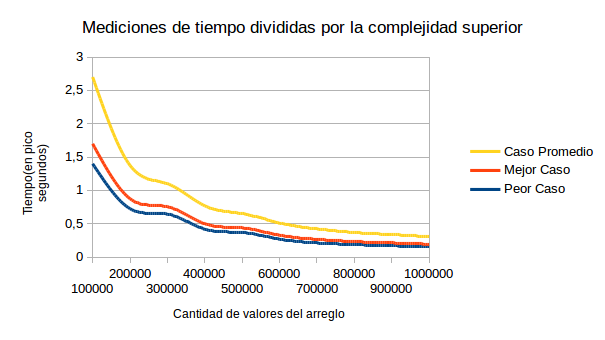
\includegraphics[width=1.1\textwidth]{imagenes/Experimento2Ej2.png}
  \caption{Tiempos de ejecución sobre complejidad teórica superior}
\end{figure}

Con este segundo gráfico se pretende mostrar de forma experimental que la complejidad es correcta. El propio enunciado pedía una complejidad menor a O($n^2$), entonces
para mostrar que se cumple simplemente dividiremos los resultados de cada uno de los tiempos por el tamaño de la muestra al cuadrado. Podemos ver que para los tres casos
la función parece tender a 0 y esto nos da la idea que el algoritmo es mejor que O($n^2$).
